\documentclass{ppig}
\usepackage{epsfig, graphicx} % support for image encoding and manipulation
\usepackage{ucs} % support for using UTF-8 as input encoding in LaTeX
\usepackage[utf8x]{inputenc} % required for UTF-8 support with ucs.sty
\usepackage{tabularx, multirow, booktabs} % support for high-quality tables
\usepackage{csquotes} % support for block quotes (using displayquote command)
\usepackage{enumitem} % support for custom enumeration formats
\let\cite\shortcite % use short-form (first author et al.) for citations


% The titlebox defines how much vertical space is given for
% the authors' list. If you need extra space to show all the
% authors, uncomment the line below and increase the value. Please
% do not make the titlebox smaller than the original size of 5cm.
%\setlength\titlebox{5cm}

%\title{An Examination of IDE Design for Programming as Problem-Solving}
\title{Towards an IDE to Support Programming as Problem-Solving}

% List the authors like you would in a table.
% The \And command creates another author's column. Use it after the
% details of one author to separate them from the following author horizontally.
% The \AND command creates a new "row" of authors and it should be used
% when the authors don't fit on the same line. You may have to increase
% the titlebox so that the author's don't overlap with the abstract.
\author{Nicholas Nelson \\
  Electrical Engineering \&\\ Computer Science \\
  Oregon State University \\
  nelsonni@oregonstate.edu \\
  \And
  Anita Sarma \\
  Electrical Engineering \&\\ Computer Science \\
  Oregon State University \\
  Anita.Sarma@oregonstate.edu \\
  \And
  André van der Hoek \\
  Department of Informatics \\
  University of California, Irvine \\
  andre@ics.uci.edu
}
  
\date{\today}

% Packages and macros for editorial purposes. Not required for submission.
\usepackage{color}
\definecolor{darkgreen}{rgb}{0.0, 0.5, 0.0}
\definecolor{ballblue}{rgb}{0.13, 0.67, 0.8}
\definecolor{aoblue}{rgb}{0.0, 0.0, 1.0}
\newcommand{\bold}[1]{\textit{\textbf{\color{aoblue}#1}}} % macro for boldifications
\newcommand{\todo}[1]{\textit{\textbf{\color{red}TODO: #1}}} % macro for TODO items
\newcommand{\discuss}[1]{\textit{\textbf{\color{darkgreen}#1}}} % macro for in-line discussions/questions
\newcommand{\nameUI}{\textit{<Insert Name>} UI} % macro placeholder for the name of the UI
\usepackage{enumitem}

\begin{document}
\maketitle
\thispagestyle{empty}

\begin{abstract}

Programming is inherently a problem-solving exercise: A programmer has to create an understanding of the situation, externalize and contextualize thoughts \& ideas, develop strategies on how to proceed with the task, enact changes according to the most appropriate strategy, and reflect to learn from each problem.
Therefore, programming is clearly more than just code input, testing, and maintenance.
Current Integrated Development Environments (IDE), however, largely focus on the "writing code" parts of programming.
In this paper, we revisit which activities and actions constitute programming, and highlight six challenges to supporting these activities. 
We then briefly describe a new paradigm of interacting with the IDE that we are working on to more directly support each of the six activities. 
\end{abstract}

\section{Programming as Problem-Solving}\label{intro}
Programming is more than dealing with language syntax and semantics: it is inherently an exercise in problem-solving that extends beyond the act of editing code in an Integrated Development Environment (IDE).
We are not the first to observe this.
For instance, programming has been characterized as an iterative process of refining mental representations of computational problems and solutions and expressing those representations as code~\cite{loksa2016programming}.
Other studies have found evidence for the facts that programming requires gathering information from multiple sources~\cite{sillito2008asking}, includes creating mental models of program structures~\cite{von1995comprehension}, and involves exploring and evaluating many alternatives~\cite{hartmann2008design}.

% Much is known already about programming being a problem-solving activity beyond editing code in the editor provided by the IDE.
% During software development, for instance, programmers are known to create all sorts of auxiliary non-code artifacts~\cite{cherubini2007whiteboard}.
% As a second example, programmers are known to organize these artifacts into structures that are relevant to the particular task(s) they are currently focused upon~\cite{baltes2016empirical}.
% As a final example, programmers are known to not pursue a single solution, but to generally approach a task by exploring (either mentally or externalized) multiple alternative solutions~\cite{madeyski2017experimentation}.
% By applying prior work on problem-solving from a cognitive psychology perspective~\cite{mayer1992thinking}, we can classify these actions, respectively, into \textit{representing relevant information}, \textit{contextualizing information}, and \textit{generating alternatives}.
% These actions can then be generalized to represent the problem-solving activities of \textit{externalizing thoughts \& ideas} and \textit{developing strategies}.

We surveyed the literature from the perspective of programming as problem-solving, with Table~\ref{pps_matrix} summarizing key activities that developers employ when programming. These activities can be partitioned into six categories (\textit{Activities}), with specific actions that represent in more detail how the high-level activities manifest themselves in practice (\textit{Actions}).
Clearly, not every task involves all of these problem-solving actions, and there is no linearity to the order in which they are employed.
Sometimes an action may not even be observable when it takes place solely in a programmer's head.
At the same time, literature has documented that all of these actions do occur and play an important role in how programmers arrive at a solution to the programming problem at hand.

\begin{table}[!htbp]
\caption{Activities and Actions of Programming as Problem-Solving}
\label{pps_matrix}
\centering
\begin{tabular}{|c|c|l|}
	\hline
	\multicolumn{2}{|c|}{\textbf{Activities}} & \multicolumn{1}{|c|}{\textbf{Actions}}\\\hline
	\multirow{5}{*}{A1} & \multirow{5}{*}{Understanding the situation} & Identifying goals \\
		& & Recalling prior knowledge \\
		& & Constructing models \\
		& & Interpreting code artifacts \\
		& & Filling knowledge gaps \\\hline
	\multirow{3}{*}{A2} & \multirow{3}{*}{Externalizing thoughts \& ideas} & Representing relevant information \\
		& & Contextualizing information \\
		& & Preserving contextual information \\\hline
	\multirow{4}{*}{A3} & \multirow{4}{*}{Developing strategies} & Generating alternatives \\
		& & Articulating and refining alternatives \\
		& & Understanding and assessing alternatives \\
		& & Recombining aspects of alternatives \\\hline
	\multirow{3}{*}{A4} & \multirow{3}{*}{Enacting change} & Translating strategies to actions \\
		& & Tracking progress \\
		& & Evaluating and assessing change \\\hline
	\multirow{5}{*}{A5} & \multirow{5}{*}{Collaborate} & Feedback solicitation \\
		& & Team work \\
		& & Group think \\
		& & Leverage group knowledge \\
		& & Synchronization \\\hline
	\multirow{2}{*}{A6} & \multirow{2}{*}{Retrospect} & Reflect on work \\
		& & Preserve work \\\hline
\end{tabular}
\end{table} % Programming as Problem-Solving Matrix

\section{Challenges}\label{challenges}
We believe that it is necessary to fundamentally rethink IDEs, so that they seamlessly and intrinsically
support programming as problem solving. Supporting the full set of actions comprising problem-solving
in programming, however, involves numerous challenges that must be addressed. These challenges span
all six categories of activities, and even those activities that have traditionally been supported by IDEs \textit{(A4)} exhibit gaps when reviewed through the lens of problem-solving requirements.

\begin{enumerate}
	\item \textit{\textbf{How to support programmers' formulation of problems and reflection on potential solutions?}}
	Programmers do not just arrive at a solution out of nowhere.
	They need to first contextualize the computational problem in terms of what they know and how they can progress towards a possible solution.
	This involves exploration, articulation, and reflection on different alternatives, with these actions being interleaved, sometimes even happening at the same time (e.g., developers are known to reflect on a code solution while they articulate it) and typically encompassing several relatively quick iterations.
	Often there is no single correct solution, and the best solution requires mixing and matching elements from multiple alternative solutions.
    
    \item \textit{\textbf{How to provide programmers access to the relevant context in a problem space?}}
    Programming solutions must exist in the context of the rest of the codebase and its related artifacts.
    Programmers need to understand where a code snippet fits in a code base, what it calls out to, and what calls into it~\cite{desouza2008empirical}, the desired behaviors of the existing codeand the code to be produced (e.g., computational speed, usability, features), organizational policies (e.g., licensing, process standards, code style), and historical development (e.g., has a solution previously been tried and rejected).
    Information that defines this context is not always readily available and, instead, must be cobbled together from multiple different types of and sources of artifacts.
    A developer needs to know where these individual pieces of information reside and how to obtain just those items that actually pertain to the problem at hand.
    
 	\item \textit{\textbf{How to support different information processing style and workflow of programmers?}}
 	Programing is a creating activity; no two programmers arrive at the same solution in the same way. For example, female programmers tend to process information comprehensively, seeking a more complete understanding of the problem before starting~\cite{grigoreanu2012end}, whereas male programmers are known to use a more heuristic (or selective) approach. As another example, visuospatial reasoning is critical for abstract knowledge and inference, and is a core component of how we view the world, but it has been observed that programmers bring their own personal visuospatial reasoning and information processing style to evaluating and organizing artifacts, solutions, and ideas~\cite{tversky2005visuospatial}.
  
  \item \textit{\textbf{How to support programmers in relying on past experience?}}
  Problem-solving in programming is not a one-off activity performed in isolation.
  Instead, programmers rely upon past experiences with similar problems, knowledge gained from previous artifact interactions, and prior mental models. % that allowed comprehension and problem-solving to succeed. 
  The question arises of how this prior experience can be brought to bear, easily, when a programmer faces a new situation. Apart from the programmer memorizing what they might have done in the past and looking this up, current IDEs provide no support in this regard. The challenge lies in how a new IDE can provide this kind of assistance.
% When solving a programming problem, programmers need to orient around both their own and others' problem-solving spaces in order to transition from contemplating into actualizing (enacting) a solution.
  
  \item \textit{\textbf{How to enable collaboration between programmers across all artifacts involved in problem solving?}}
As already highlighted, programmers contextualize their work with all sorts of different artifacts. Yet, current IDEs generally only allow sharing of the code being worked on. Successful collaboration, however, requires sharing of all different artifacts so all participants have access to the full context. Moreover, it requires ongoing programmers to  know how their changes may affect others, and who may be making changes that affect their own work ~\cite{desouza2008empirical}. Finally, they also need to understand the provenance of design decisions, and how and why these decisions were made. 

\item \textit{\textbf{How to utilize different pieces of information and context to support the act of coding?}}
Solutions to computation problems must eventually be represented in code.
Converting a conceptual solution into actual lines of code is a non-linear activity (coding sessions start and stop), occurs concurrently with other problem-solving activities, and is loosely organized (e.g., solutions are partially implemented, abandoned, and recovered).
Creating a simple, elegant software solution hinges on complex, exploratory coding sessions, and the IDE must support this process fluidly.

%Therefore, programmers must cope with high-complexity coding sessions in the pursuit of simple, elegant software solutions.
\end{enumerate}

\section{Toward A New IDE}\label{new_ide}
To address these challenges, we have begun a research effort that attempts to rethink the IDE from the ground up using a problem-solving perspective for evaluating our design rationale.
We use Code Bubbles~\cite{bragdon2010bubbles}, Code Canvas~\cite{deline2010canvas}, and Patchworks Code Editor~\cite{henley2014patchworks} as key inspirations for interface designs that eschew window-based interfaces and explore spatial interfaces allowing users to project meaning onto the layout of their development environment.
We also rely upon Lighthouse~\cite{dasilva2006lighthouse} as an inspiration for parallel development awareness in interface design.
Extending the zoomable canvas of Code Canvas and the bubble windows of Code Bubbles, plus the live information of Lighthouse, we explore these and other concepts from interface design to support the problem-solving activities that programmers encounter.

\vspace*{-0.3\baselineskip}
\begin{figure}[h!]
	\caption{Cards-based User Interface of a Problem-Solving IDE}
	\label{mockup}
    \centering
	% trim={<left> <lower> <right> <upper>}	
    \fbox{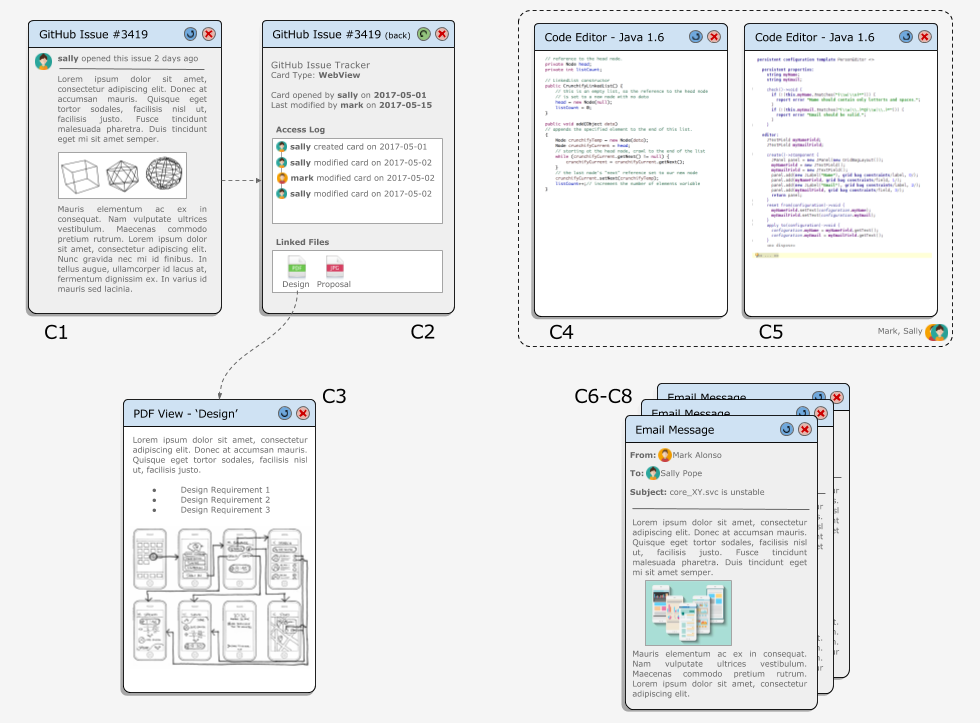
\includegraphics[trim={0.6cm 0.2cm 0.6cm 0.2cm},clip,width=0.9\textwidth]{Mockup-10}}
	\vspace*{-0.4\baselineskip}
\end{figure}

Figure~\ref{mockup} provides a high-fidelity illustration of our proposed user interface for a new IDE that allows user-driven problem-solving to occur natively within a single environment.
As shown in Figure~\ref{mockup}, we propose a cards-based user interface so that developers can take advantage of the neuro-cognitive process of perceptual organization~\cite{kimchi2003perceptual}.
Spatial perception allows developers to provide meaning to individual artifacts (i.e., cards) by organizing them in patterns that contextualize the individual artifact, its relation to other artifacts, and the larger purpose.
As previously demonstrated, developers work with artifacts beyond code and therefore require cards that accommodate those non-code artifacts.
We propose cards of different types to address different problem-solving aspects: code editor cards for code artifacts (cards \texttt{C4}, \texttt{C5}), issue tracker cards for problem contextualization (\texttt{C1}, \texttt{C2}), image and PDF cards for design documents (\texttt{C3}), or email viewer cards for communications (\texttt{C6-C8}).
This list is not exhaustive, and we expect that additional card types will be proposed and developed to accommodate additional problem-solving activities.

Individual cards can be stacked together into logical units of meaning based upon the programming problem and the developer's approach to it (e.g. cards \texttt{C6-C8}).
This flexibility allows cards of different types to be stacked into groups that are relevant to the current task, and then unstacked and stacked again for subsequent tasks.
Since developers work together, in a variety of different capacities (see Table~\ref{pps_matrix} -- A5), we also propose integrated methods for sharing individual cards (or stacks of cards) for either review or simultaneous editing.
This feature can be seen in cards ~\texttt{C4} and \texttt{C5}, which are shown as being shared between two different developers to allow them to discuss and modify the cards as needed to address a programming problem.

Our proposed cards-based IDE attempts to address each of the six problem-solving activities (Table~\ref{pps_matrix}) through the use of cards that allow for the construction and interpretation of artifacts related to the situation (A1), the creation of new contextually relevant cards (A2), the organization of cards in stacks to explore and refine solutions (A3), the ability to directly edit code and other artifacts (A4), the ability to share and synchronization development between individual developers (A5), and to reflect upon and preserve desirable solutions (A6).

\bibliography{bibliography}
\bibliographystyle{apacite}
\end{document}
